\section{Analysis}\label{sec:analysis}
In this section, we prove the security of our scheme. Before we delve in detail into the formal
details of the proof, let us first observe why the $1/4$ bound is necessary through a combined attack
on our construction.

After the suggested protocol update the honest prover cannot include any thorny blocks in his suffix NIPoPoW even if these blocks are part of his chain $\chain_B$. The adversary may exploit this fact as follows. She tries to suppress high-level honestly generated blocks in $\chain_B$, in order to reduce the blocks that can represent the honest chain in a proof. This can be done by mining a \emph{suppressive block} on the parent of an honest superblock on the honest chain and hoping that she will be faster than the honest parties. In parallel, while she mines suppressive thorny blocks on $\chain_B$ she can still use her blocks in her NIPoPoW proofs, by chainsewing them. Consequently, even if a suppression attempt does not succeed, in case for example a second honestly generated block is published soon enough, she does not lose the mining power spent but can still utilize it by including the block in her proof.

In more detail, consider the adversary who wishes to attack a specific block level $\mu_B$ and generates a NIPoPoW proof containing a block $b$ of a fork chain which contains a double spending transaction. Then she acts as follows. She mines on her fork chain $\chain_\mathcal{A}$ but when she observes a $\mu_B$-level block in $\chain_B$ she tries to mine a thorny block on $\chain_B$ in order to suppress this $\mu_B$ block. This thorny block contains an interlink pointer which jumps onto her fork chain, but a previd pointer to the honest chain. If the suppression succeeds she has managed to damage the distribution of $\mu_B$-superblocks within the honest chain, at the same time, to mine a block that she can afterwards use in her proof. If the suppression does not succeed she can still use the thorny block in her proof. The above are illustrated in Figure~\ref{fig:attack_after_update}.

\begin{figure}
    \begin{center}
        \iftwocolumn
            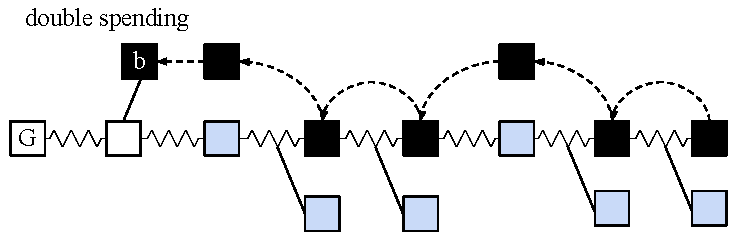
\includegraphics[width=0.95\columnwidth]{figures/attack_after_update-crop.pdf}
        \else
            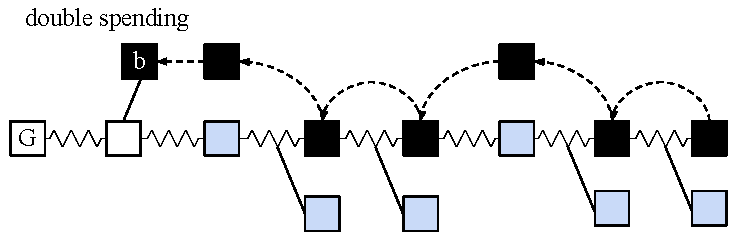
\includegraphics[width=0.6\columnwidth]{figures/attack_after_update-crop.pdf}
        \fi
	\end{center}
	\caption{The adversary suppresses honestly generated blocks and chainsews thorny blocks in $\chain_B$. Blue blocks are honestly generated blocks of some level of attack. The adversary tries to suppress them. If the suppression is not successful, the adversary can still use the block she mined in her proof.}
	\label{fig:attack_after_update}
\end{figure}

The described attack is a combined attack which combines both superblock suppression (initially described in~\cite{nipopows}, a variant of selfish mining~\cite{selfish}) and chainsewing (introduced in this work). This combined attack forces us to consider the Velvet Honest Majority Assumption of (1/4)-bounded adversary, so as to guarantee that the unsuppressed blocks in $\chain_B$ suffice for constructing winning NIPoPoW proofs against the adversarial ones.

For the analysis, we use the techniques
developed in the Backbone line of work~\cite{backbone}. Towards that end, we
follow their definitions and call a round \emph{successful} if at least one
honest party made a successful random oracle query during the round, i.e., a
query $b$ such that $H(b) \leq T$. A round in which exactly one honest party
made a successful query is called \emph{uniquely successful} (the adversary
could have also made successful queries during a uniquely successful round). Let
$X_r \in \{0, 1\}$ and $Y_r \in \{0, 1\}$ denote the indicator random variables
signifying that $r$ was a successful or uniquely successful round respectively,
and let $Z_r \in \mathbb{N}$ be the random variable counting the number of
successful queries of the adversary during round $r$. For a set of consecutive
rounds $U$, we define $Y(U) = \sum_{r \in U} Y_r$ and similarly define $X$ and
$Z$. We denote $f = \Ex[X_r] < 0.3$ the probability that a round is successful.

Let $\lambda$ denote the security parameter (the output size $\kappa$ of the
random oracle is taken to be some polynomial of $\lambda$).
We make use of the following known~\cite{backbone} results.
It holds that $pq(n-t) < \dfrac{f}{1-f}$. For the Common Prefix
parameter, it holds that $k \geq 2\lambda f$.
Additionally, for any set of
consecutive rounds $U$, it holds that
$\Ex[Z(U)] < \frac{t}{n-t} \cdot \frac{f}{1 - f}|U|$,
$\Ex[X(U)] < pq(n - t)|U|$,
$\Ex[Y(U)] > f(1 - f)|U|$.
An execution is called \emph{typical}
if the random variables $X, Y, Z$ do not deviate significantly (more than some
error term $\epsilon < 0.3$) from their expectations. It is known that
executions are typical with overwhelming probability in
$\lambda$. Typicality ensures that for any set of consecutive
rounds $U$ with $|U| > \lambda$ it holds that
$Z(U) < \Ex[Z(U)] - \epsilon\Ex[X(U)]$ and
$Y(U) > (1 - \epsilon)\Ex[Y(U)]$.
From the above we can conclude to
$Y(U) > (1 - \epsilon)f(1-f) \lvert U \rvert$ and
$Z(U) < \dfrac{t}{n-t} \cdot \dfrac{f}{1-f} \lvert U \rvert + \epsilon f \lvert U \rvert $ which will be used in our proofs.
We consider $f < \dfrac{1}{20}$ a typical bound for parameter $f$. This is because in our (1/4)-bounded adversary assumption we need to reach about 75\% of the network, which requires about 20 seconds~\cite{Wattenhofer}. Considering also that in Bitcoin the block generation time is in expectation 600 seconds, we conclude to an estimate $f = \dfrac{18}{600}$ or $f = 0.03$.

The following definition and lemma are known~\cite{dionyziz} results and will
allow us to argue that some smooth superblocks will survive in all honestly
adopted chains. With foresight, we remark that we will take $Q$ to be the
property of a block being both smooth and having attained some superblock level
$\mu \in \mathbb{N}$.

\begin{definition}[$Q$-block]
    A \emph{block property} is a predicate $Q$ defined on a hash output $h \in \{ 0, 1 \}^\kappa$. Given a block property $Q$, a valid block with hash $h$ is called a $Q$-block if $Q(h)$ holds.
\end{definition}

\begin{lemma}[Unsuppressibility]
    Consider a collection of polynomially many block properties $\mathcal{Q}$. In a typical execution every set of consecutive rounds $U$ has a subset $S$ of uniquely successful rounds such that
    \begin{itemize}
        \item $\lvert S \rvert \geq Y(U) - 2Z(U) - 2 \lambda f (\dfrac{t}{n-t} \cdot \dfrac{1}{1-f} + \epsilon)$
        \item for any $Q \in \mathcal{Q}$, $Q$-blocks generated during $S$ follow the distribution as in an unsuppressed chain
        \item after the last round in $S$ the blocks corresponding to $S$ belong
        to the chain of any honest party.
    \end{itemize}
\end{lemma}

We now apply the above lemma to our construction. The following result lies at
the heart of our security proof and allows us to argue that an honestly adopted
chain will have a better superblock score than an adversarially generated chain.

\begin{lemma}\label{lem:claim3_lemma}
   Consider Algorithm \ref{alg:updateInterlink} under velvet fork with parameter $g$ and (1/4)-bounded velvet honest majority. Let $U$ be a set of consecutive rounds $r_1 \cdots r_2$ and $\chain$ the chain of an honest party at round $r_2$ of a typical execution. Let $\chain^S_U = \{b \in \chain: \text{b is smooth} \land \text{b was generated during U} \}$. Let $\mu, \mu' \in \mathbb{N}$.
   Let $\chain'$ be a $\mu'$ superchain containing only adversarial blocks generated during $U$ and suppose $\lvert \chain^S_U\upchain^{\mu} \rvert > k$. Then for any $\delta_3 \leq \dfrac{3\lambda f}{5} $ it holds that
   $2^{\mu'}\lvert \chain' \rvert < 2^{\mu} ( \lvert \chain^S_U\upchain^{\mu} \rvert + \delta_3 )$.
\end{lemma}
\begin{proof}
  From the Unsuppressibility Lemma we have that there is a set of uniquely
  successful rounds $S \subseteq U$, such that
  $\lvert S \rvert \geq Y(U) - 2Z(U) - \delta'$, where
  $\delta' = 2 \lambda f (\dfrac{t}{n-t} \cdot \dfrac{1}{1-f} + \epsilon)$.
  We also know that $Q$-blocks generated during $S$ are distributed as in an
  unsuppressed chain. Therefore considering the property $Q$ for blocks of
  level $\mu$ that contain smooth interlinks we have that
  $\lvert \chain^S_U\upchain^{\mu} \rvert \geq (1-\epsilon)g2^{-\mu} \lvert S \rvert$.
  We also know that for the total number of $\mu'$-blocks the adversary
  generated during $U$ that
  $\lvert \chain' \rvert \leq (1+\epsilon)2^{-\mu'}Z(U)$.
  Then we have to show that
  $(1-\epsilon)g (Y(U) - 2Z(U) - \delta' ) > (1+\epsilon)Z(U)$ or
  $((1+\epsilon)+2g(1-\epsilon))Z(U) < g(1-\epsilon)(Y(U) + \delta')$.
  But it holds that $ (1+\epsilon)+2g(1-\epsilon) < 3$, therefore it suffices to show that
  $3Z(U) < g(1-\epsilon)(Y(U) + \delta') - 2^\mu \delta_3$.

Substituting the bounds of $X$, $Y$, $Z$ discussed above, it suffices to show that
\begin{equation*}
    3[\dfrac{t}{n-t} \cdot \dfrac{f}{1-f} \lvert U \rvert + \epsilon f \lvert U \rvert ] < (1- \epsilon)g[ (1-\epsilon)f(1-f) \lvert U \rvert - \delta'] - 2^\mu \delta_3
\end{equation*} or
%\begin{equation*}
%        3f \lvert U \rvert \dfrac{f}{1-f}\cdot \dfrac{t}{n-t} + 3 \epsilon f \lvert U \rvert < (1- \epsilon)g[ (1-\epsilon)f(1-f) \lvert U \rvert - \delta'] -2^\mu \delta_3
%\end{equation*} or
%\begin{equation*}
%        \dfrac{t}{n-t} < \dfrac{ (1- \epsilon)g[ (1-\epsilon)f(1-f) \lvert U \rvert - \delta' ] - 3\epsilon f \lvert U \rvert -2^\mu \delta_3 }  { 3 \dfrac{f}{1-f} \lvert U \rvert}
%\end{equation*} or
$\dfrac{t}{n-t} < \dfrac{  (1- \epsilon)g[ (1-\epsilon)f(1-f) - \dfrac{\delta'}{\lvert U \rvert} ] - 3 \epsilon f - \dfrac{2^\mu \delta_3}{\lvert U \rvert} }  { 3\dfrac{f}{1-f}}$.

But $\epsilon(1-f) \ll 1$
thus we have to show that
%\begin{equation*}
%    \dfrac{t}{n-t} < \dfrac{  (1- \epsilon)g[ (1-\epsilon)f(1-f) - \dfrac{\delta'}{\lvert U \rvert} ] - \dfrac{2^\mu \delta_3}{\lvert U \rvert} }  { 3 \dfrac{f}{1-f}} - \epsilon'
%\end{equation*} or
\begin{equation}\label{eq:lemma_eq1}
    \dfrac{t}{n-t} < \dfrac{g}{3} \cdot \dfrac{(1-\epsilon)^2 f(1-f) - \dfrac{(1-\epsilon)\delta'}{\lvert U \rvert} - \dfrac{2^\mu \delta_3}{\lvert U \rvert} }{\dfrac{f}{1-f}} - \epsilon'
\end{equation}

In order to show Equation~\ref{eq:lemma_eq1} we use $f \leq \dfrac{1}{20}$ which is a typical bound for our setting as discussed above.
Because all blocks in $\chain$ were generated during $U$ and $\lvert \chain \rvert > k $, $\lvert U \rvert$ follows negative binomial distribution with probability $2^{-\mu} pq(n-t)$ and number of successes $k$.
Applying a Chernoff bound we have that $\lvert U \rvert > (1-\epsilon) \dfrac{k}{2^{-\mu} pq(n-t)}$. Using the inequalities $k \geq 2\lambda f$ and $pq(n-t) < \dfrac{f}{1-f}$, we deduce that $\lvert U \rvert > (1-\epsilon) 2^{\mu}2\lambda(1-f)$. So we have that $\dfrac{\delta'}{\lvert U \rvert} < \dfrac{2\lambda f (\dfrac{t}{n-t} \dfrac{1}{1-f} + \epsilon)}{(1-\epsilon)2^{\mu}2\lambda (1-f)}$ or $\dfrac{\delta'}{\lvert U \rvert} < \dfrac{t}{n-t} \cdot \dfrac{f}{(1-\epsilon)(1-f)^2} + \epsilon < 0.01 + \epsilon$.
We also know that $\delta_3 \leq \dfrac{ 3\lambda f}{5}$, so
$\dfrac{2^{\mu} \delta_3}{\lvert U \rvert} < \dfrac{2^\mu \dfrac{ 3\lambda f}{5}}{2^{\mu} 2 \lambda (1-f)}$ or
$\dfrac{2^{\mu} \delta_3}{\lvert U \rvert} < \dfrac{3f}{10(1-f)} < 0.01 + \epsilon$.
By substituting the above and the typical $f$ parameter bound in Equation (\ref{eq:lemma_eq1}) we conclude that it suffices to show that $\dfrac{t}{n-t} < \dfrac{1-\epsilon''}{3}g$
which is equivalent to $\dfrac{t}{n-t} < \dfrac{1-\delta_v}{3}g$ for $\epsilon'' = \delta_v$, which is the (1/4) velvet honest majority assumption, so the claim is proven.
\end{proof}

\begin{lemma}\label{lem:claim1_lemma}
    Consider Algorithm \ref{alg:updateInterlink} under velvet fork with parameter $g$ and (1/4)-bounded velvet honest majority. Consider the  property $Q$ for blocks of level $\mu$. Let $U$ be a set of consecutive rounds and $\chain$ the chain of an honest party at the end of $U$ of a typical execution and $\chain_U = \{ b \in \chain: \text{b was generated during U} \}$. Suppose that no block in $\chain_U$ is of level $\mu$. Then $\lvert U \rvert \leq \delta_1$ where
    $\delta_1 = \dfrac{(2+\epsilon) 2^{\mu} + \delta'}{(1-\epsilon)f(1-f) - 2\dfrac{t}{n-t}\dfrac{f}{1-f} -3\epsilon f}$.
\end{lemma}
\begin{proof}
    The statement results immediately form the Unsuppressibility Lemma. Suppose for contradiciton that $\lvert U \rvert > \delta_1 $.
    Then from the Unsuppressibility Lemma we have that there is a subset of consecutive rounds $S$ of $U$ for which it holds that
    $\lvert S \rvert \geq Y(U) - 2Z(U) - \delta'$ where
    $\delta' = 2 \lambda f (\dfrac{t}{n-t} \cdot \dfrac{1}{1-f} + \epsilon)$. By substituting
    $Y(U) > (1-\epsilon)f(1-f) \lvert U \rvert$ and
    $Z(U) < \dfrac{t}{n-t} \dfrac{f}{1-f} +\epsilon f \lvert U \rvert$ we have that $\lvert S \rvert > (2+\epsilon)2^{\mu}$ but $Q$-blocks generated during $S$ follow the distribution as in a chain where no suppression attacks occur. Therefore at least one block of level $\mu$ would appear in $\chain_U$, thus we have reached a contradiction and the statement is proven.
\qed
\end{proof}

\begin{theorem}[Suffix Proofs Security under velvet fork]
	Assuming honest majority under velvet fork conditions (\ref{defn:velvet_honest_majority}) such that $t \leq (1 - \delta_v) \dfrac{n_h}{3}$ where $n_h$ the number of upgraded honest parties, the Non-Interactive Proofs of Proof-of-Work construction for computable $k$-stable monotonic suffix-sensitive predicates under velvet fork conditions in a typical execution is secure.
\end{theorem}
\begin{proof}
By contradiction. Let $Q$ be a $k$-stable monotonic suffix-sensitive chain predicate. Assume for contradiction that NIPoPoWs under velvet fork on $Q$ is insecure. Then, during an execution at some round  $r_3$, $Q(\chain)$ is defined and the verifier $V$ disagrees with some honest participant. $V$ communicates with adversary $\mathcal{A}$ and honest prover $B$. The verifier receives proofs $\pi_\mathcal{A}, \pi_B$ which are of valid structure. Because $B$ is honest, $\pi_B$ is a proof constructed based on underlying blockchain $\chain_B$ (with $\pi_B \subseteq \chain_B$), which $B$ has adopted during round $r_3$ at which $\pi_B$ was generated. Consider $\widetilde{\chain}_\mathcal{A}$ the set of blocks defined as $\widetilde{C}_\mathcal{A} = \pi_\mathcal{A} \cup \{ \bigcup \{\chain_h^r\{{:}b_\mathcal{A}\}:  b_\mathcal{A} \in \pi_\mathcal{A}, \exists h,r : b_\mathcal{A} \in \chain_{h}^{r}\}  \}$ where $\chain_h^r$ the chain that the honest party $h$ has at round $r$. Consider also $\chain^S_B$ the set of smooth blocks of honest chain $\chain_B$. We apply security parameter
\begin{equation*}
    m = 2k + \dfrac{2+\epsilon + \delta'}{\dfrac{t}{n-t}\dfrac{f}{1-f}[f(1-f) - \dfrac{2}{3}\dfrac{f}{1-f}]}
\end{equation*}

Suppose for contradiction that the verifier outputs $\neg Q(\chain_B)$. Thus it is necessary that $\pi_\mathcal{A} {\geq}_m \pi_B$. We show that $\pi_\mathcal{A} {\geq}_m \pi_B$ is a negligible event.
Let the levels of comparison decided by the verifier be $\mu_\mathcal{A}$ and $\mu_B$ respectively. Let $b_0 = LCA(\pi_\mathcal{A}, \pi_B)$. Call $\alpha_\mathcal{A} = \pi_\mathcal{A} \upchain^{\mu_\mathcal{A}}\{b_0{:}\}$, $\alpha_B = \pi_B \upchain^{\mu_B}\{b_0{:}\}$.

From Lemma~\ref{lem:adversarial_proof_scheme} we have that the adversarial proof consists of a smooth interlink subchain followed by a thorny interlink subchain. We refer to the smooth part of $\alpha_\mathcal{A}$ as $\alpha^{\mathcal{S}}_\mathcal{A}$ and to the thorny part as $\alpha^{\mathcal{T}}_\mathcal{A}$.

Our proof construction is based on the following intuition: we consider that $\alpha_\mathcal{A}$ consists of three distinct parts $\alpha_\mathcal{A}^1, \alpha_\mathcal{A}^2, \alpha_\mathcal{A}^3$ with the following properties.
Block $b_0 = LCA(\pi_\mathcal{A}, \pi_B)$ is the fork point between $\pi_\mathcal{A} \upchain^{\mu_\mathcal{A}}, \pi_B \upchain^{\mu_B}$. Let block $b_1 = LCA (\alpha^{\mathcal{S}}_\mathcal{A}, \chain^S_B)$ be the fork point between $\pi^{\mathcal{S}}_\mathcal{A} \upchain^{\mu_\mathcal{A}}, \chain_B $ as an honest prover could observe. Part $\alpha_\mathcal{A}^1$ contains the blocks between $b_0$ exclusive and $b_1$ inclusive generated during the set of consecutive rounds $\mathcal{S}_1$ and $\lvert  \alpha_\mathcal{A}^1 \rvert = k_1$. Consider $b_2$ the last block in $\alpha_\mathcal{A}$ generated by an honest party. Part $\alpha_{\mathcal{A}}^2$ contains the blocks between $b_1$ exclusive and $b_2$ inclusive generated during the set of consecutive rounds $\mathcal{S}_2$ and $\vert  \alpha_\mathcal{A}^2 \vert = k_2$. Consider $b_3$ the next block of $b_2$ in $\alpha_\mathcal{A}$. Then $\alpha_{\mathcal{A}}^3 = \alpha_\mathcal{A}[b_3{:}]$ and $\vert  \alpha_\mathcal{A}^3 \vert = k_3$ consisting of adversarial blocks generated during the set of consecutive rounds $\mathcal{S}_3$. Therefore $\vert \alpha_\mathcal{A} \vert = k_1 + k_2 + k_3$ and we will show that $\vert \alpha_\mathcal{A} \vert < \vert \alpha_B \vert$.

The above are illustrated, among other, in Parts I, II of Figure \ref{fig:proof_velvet}.

\begin{figure}
    \begin{center}
        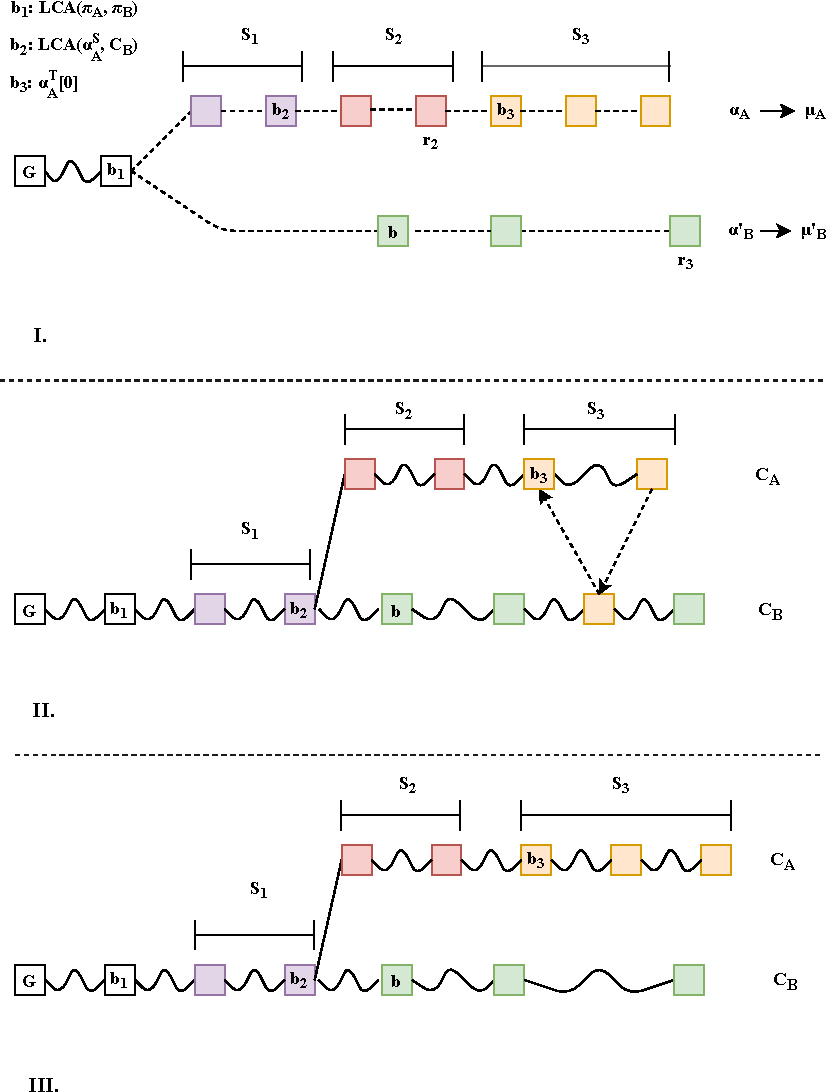
\includegraphics[width=0.95 \columnwidth]{figures/proof_velvet-crop.pdf}
    \end{center}
    \caption{I. the three round sets in two competing proofs at different levels, II. the corresponding 0-level blocks implied by the two proofs, III: blocks in $\chain_B$ and block set $\widetilde{\chain}_\mathcal{A}$ from the verifier's perspective.}
    \label{fig:proof_velvet}
\end{figure}

We now show three successive claims: First that $\alpha_\mathcal{A}^1$ contains few blocks. Second, $\alpha_\mathcal{A}^2$ contains few blocks. And third, the adversary can produce a winning $a_\mathcal{A}$ with negligible probability.

\textbf{Claim 1:} \textit{$\alpha_\mathcal{A}^1 = (\alpha_\mathcal{A}\{b_0 : b_1\} \cup b_1)$ contains only a few blocks.} Let $\lvert \alpha^1_\mathcal{A} \rvert = k_1$. We have defined the blocks $b_0 = LCA(\pi_\mathcal{A}, \pi_B)$ and $b_1 = LCA(\alpha^{\mathcal{S}}_\mathcal{A}, \chain^S_B)$. First observe that because of the Lemma~\ref{lem:adversarial_proof_scheme} there are no thorny blocks in $\alpha_\mathcal{A}^1$ since $\alpha_\mathcal{A}^1[-1] = b_1$ is a smooth block. This means that if $b_1$ was generated at round $r_{b_1}$ and $\alpha^{\mathcal{S}}_\mathcal{A}[-1]$ in round $r$ then $r \geq r_{b_1}$. Therefore, $\alpha_\mathcal{A}^1$ contains smooth blocks of $\chain_B$. We show the claim by considering the two possible cases for the relation of $\mu_\mathcal{A}, \mu_B$.

\textit{\underline{Claim 1a}:} \textit{If $\mu_B \leq \mu_\mathcal{A}$ then $k_1 = 0$}. In order to see this, first observe that every block in $\alpha_\mathcal{A}$ would also be of lower level $\mu_B$. Subsequently, any block in $\alpha_\mathcal{\mathcal{A}}\{b_0{:}\}$ would also be included in proof $\alpha_B$ but this contradicts the minimality of block $b_0$.

\textit{\underline{Claim 1b}:} \textit{If $\mu_B > \mu_\mathcal{A}$ then $k_1 \leq \dfrac{\delta_1 2^{-\mu_\mathcal{A}}}{(1+\epsilon)\dfrac{t}{n-t}\dfrac{f}{1-f}}$}. In order to show this we consider block $b$ the first block in $\alpha_B$. Now suppose for contradiction that $k_1 > \dfrac{\delta_1 2^{-\mu_\mathcal{A}}}{(1+\epsilon)\dfrac{t}{n-t}\dfrac{f}{1-f}}$. Then from lemma \ref{lem:claim1_lemma} we have that block $b$ is generated during $S_1$. But $b$ is of lower level $\mu_\mathcal{A}$ and $\alpha^1_\mathcal{A}$ contains smooth blocks of $\chain_B$. Therefore $b$ is also included in $\alpha^1_\mathcal{A}$, which contradicts the minimality of block $b_0$.

Consequently, there are at least $\lvert \alpha_\mathcal{A} \rvert - k_1$ blocks in $\alpha_\mathcal{A}$ which are not honestly generated blocks existing in $\chain_B$. In other words, these are blocks which are either thorny blocks existing in $\chain_B$ either don't belong in $\chain_B$.

\textbf{Claim 2.}
\textit{Part $\alpha_\mathcal{A}^2 = (\alpha_\mathcal{A}\{b_1:b_2\} \cup b_2)$ consists of only a few blocks.} Let $ \lvert \alpha_\mathcal{A}^2 \rvert = k_2$. We have defined $b_2 = \alpha_\mathcal{A}^2[-1]$ to be the last block generated by an honest party in $\alpha_\mathcal{A}$. Consequently no thorny block exists in $\alpha_\mathcal{A}^2$, so all blocks in this part belong in a proper zero-level chain $\chain_\mathcal{A}^2$.  Let $r_{b_1}$ be the round at which $b_1$ was generated. Since $b_1$ is the last block in $\alpha_\mathcal{A}$ which belongs in $\chain_B$, then $\chain_\mathcal{A}^2$ is a fork chain to $\chain_B$ at some block $b'$ generated at round $r' \geq r_{b_1}$. Let $r_2$ be the round when $b_2$ was generated by an honest party. Because an honest party has adopted chain $\chain_B$ at a later round $r_3$ when the proof $\pi_B$ is constructed and because of the Common Prefix property on parameter $k_2$, we conclude that $k_2 \leq 2^{-\mu_\mathcal{A}}k$.

\textbf{Claim 3.} \textit{The adversary may submit a suffix proof such that $\lvert \alpha_\mathcal{A}\rvert \geq \lvert \alpha_B \rvert$ with negligible probability.} Let $ \lvert \alpha_\mathcal{A}^3 \rvert = k_3$. As explained earlier part $\alpha^3_\mathcal{A}$ consists only of adversarially generated blocks. Let $S_3$ be the set of consecutive rounds $r_2...r_3$. Then all $k_3$ blocks of this part of the proof are generated during $S_3$. Let $\alpha^{3}_B$ be the last part of the honest proof containing the interlinked $\mu_B$ superblocks generated during $S_3$. Then by applying lemma \ref{lem:claim3_lemma} $\dfrac{m}{k}$ times we have that $ 2^{\mu_\mathcal{A}}\lvert \alpha^3_\mathcal{A} \rvert < 2^{\mu_B} (\lvert \alpha^{S_3}_{B}\upchain^{\mu_B} \rvert + \dfrac{m\delta_3}{k})$. By substituting the values from all the above Claims and because every block of level $\mu_B$ in $a\alpha_B$ is of equal hashing power to $2^{\mu_B - \mu_\mathcal{A}}$ blocks of level $\mu_\mathcal{A}$ in the adversary's proof we have that:
$2^{\mu_B} \lvert \alpha{_B^{3}} \rvert - 2^{\mu_\mathcal{A}} \lvert \alpha_\mathcal{A}^{3} \rvert > 2^{\mu_\mathcal{A}}(k_1 + k_2)$
or $2^{\mu_B} \lvert \alpha{_B^{3}} \rvert > 2^{\mu_\mathcal{A}} \lvert \alpha_\mathcal{A}^{1} + \alpha_\mathcal{A}^{2} + \alpha_\mathcal{A}^{3}\rvert $
or $2^{\mu_B} \lvert \alpha{_B} \rvert > 2^{\mu_\mathcal{A}} \lvert \alpha_\mathcal{A} \rvert $
Therefore we have proven that $2^{\mu_B} \lvert \pi_B \upchain^{\mu_B} \rvert > 2^{\mu_\mathcal{A}} \lvert \pi_\mathcal{A}^{\mu_\mathcal{A}} \rvert$.
\qed
\end{proof}
